\documentclass[11pt]{article}
\usepackage[utf8]{inputenc}

\usepackage{geometry}
\geometry{a4paper}

\usepackage{graphicx}
\usepackage{hyperref}
\usepackage[parfill]{parskip}
\usepackage{amsmath, amssymb}
\usepackage{fdsymbol}
\usepackage{color,soul}

% remove section numbering
\makeatletter
\renewcommand{\@seccntformat}[1]{}
\makeatother

% make subsubsection italic
\usepackage{sectsty}
\subsubsectionfont{\itshape}

\renewcommand{\arraystretch}{1.4}

\title{Probability Theory \& Statistics}
\date{}
\author{}

\begin{document}
\maketitle
\clearpage

\section{Random Variables \& Distributions}

\subsection{Random Variables}

\emph{Random variables}. 
A \emph{random variable} (r.v.) is a function
assigning a real number to every possible outcome of an experiment.

There are two main types of random variables used in practice:
\emph{discrete} r.v.s and \emph{continuous} r.v.s. 
Discrete r.v.s. are conceptually easier to grasp so we will start with them. 
At the end of the text, 
we briefly introduce continuous r.v.s. 
but most of the intuition needed to understand random variables and their distributions
can be gained from working with discrete random variables.

\emph{Discrete random variables}. 
A random variable \(X\) is \emph{discrete} if there is a finite list of values \(a_{1}\),
\(a_{2}\), \ldots, \(a_{n}\) or an infinite list of values \(a_{1}\),
\(a_{2}\), ... If \(X\) is a discrete random variable, then the set of
values such that \(P(X = x) > 0\) is called the \emph{support} of \(X\).

\emph{Coin tosses}. 
Consider an experiment where we toss a fair coin twice. 
The sample space, \(S\), 
consists of four possible outcomes,
\(S = \{HH,HT,TH,TT\}\). 
We list three possible random variables on this space, 
where each r.v. is a numerical summary of some aspect of the
experiment:
\begin{itemize}
\item
Let \(X\) be the number of heads. 
The r.v. \(X\) has possible values 0, 1, and 2. 
\(X\) can be seen as a function mapping the outcomes to a numerical value, 
i.e., \(X(HH) = 2\), \(X(HT) = X(TH) = 1\), and \(X(TT) = 0\)
\item
Let \(Y\) be the number of tails. 
We can express \(Y\) in terms of \(X\), 
where \(Y = 2 - X\).
\item
Let \(I\) be 1 if the first toss lands heads and 0 otherwise. 
Then \(I\) assigns the value 1 to the outcomes \(HH\) and \(HT\) and a
value 0 to the outcomes \(TH\) and \(TT\). 
The r.v. \(I\) is an example of an \emph{indicator random variable}.
\end{itemize}

\subsection{Distributions (Discrete)}

Given a random variable, 
we would like to be able to describe its
behaviour using the language of probability. 
For example, 
we might want to answer questions 
about the probability that the r.v. will fall into a given range: 
if \(L\) is the lifetime earnings of a randomly chosen company employee, 
what is the probability that \(L\) exceeds a million pounds? 
If \(M\) is the number of major earthquakes in Japan in the next five years, 
what is the probability that \(M\) equals 0? 

The \emph{distribution} of a random variable provides the answers to these questions; 
it specifies the probabilities of all events associated with the r.v., 
such as the probability of it being equal to 3 and the probability of it being at least 110.

The distribution of a discrete r.v. can be defined in several equivalent ways: 
using a \emph{probability mass function},
a \emph{cumulative distribution function},
or a \emph{story}.
For a discrete random r.v. the most natural way to define its distribution
is with a \emph{probability mass function} (PMF) which we define now.

\emph{Probability mass function}. 
The PMF of a discrete r.v. \(X\) is the function
\begin{align}
p_{X}(x)=P\left(\{X=x\}\right)=P(X=x)
\end{align}
for \(x \in \mathbb{R}\). 
The PMF is positive if \(x\) is in the support of \(X\), 0 otherwise.

\emph{Coin tosses continued}. 
We will now find the PMFs of each of the r.v.s from 
the previous section using the naïve definition of probability:%
\footnote{%
\(P(A) = |A|/|S|\), i.e., 
the probability of an event \(A\) is the number of 
favourable outcomes in \(A\) divided by
the total number of outcomes in the sample space \(S\).}

\begin{itemize}
\item
  If \(X\) is the number of heads, then.
  \begin{itemize}
  \item
    \(p_{X}(0) = P(X = 0) = 1/4\)
  \item
    \(p_{X}(1) = P(X = 1) = 1/2\)
  \item
    \(p_{X}(2) = P(X = 2) = 1/4\)
  \end{itemize}
\item
  If \(Y = 2 - X\) then
  \(P(Y = y) = P(2 - X = y) = P(X = 2 - y) = p_{X}(2 - y)\)
  \begin{itemize}
  \item
    \(p_{Y}(0) = P(Y = 0) = 1/4\)
  \item
    \(p_{Y}(1) = P(Y = 1) = 1/2\)
  \item
    \(p_{Y}(2) = P(Y = 2) = 1/4\)
  \end{itemize}
\item
  The indicator r.v. has the PMF.
  \begin{itemize}
  \item
    \(p_{I}(0) = P(I = 0) = 1/2\)
  \item
    \(p_{I}(1) = P(I = 1) = 1/2\)
  \end{itemize}
\end{itemize}

\emph{Children in UK households}. 
Let \(X\) be the number of children in 
a randomly chosen household in the UK. 
Since \(X\) can only be integer values, 
it is a \emph{discrete r.v.} 
We can approximate the proportion
of households with 0, 1, 2, ... children, 
and hence approximate the PMF of \(X\) by sampling the population.

\emph{Remark}. 
We can think of the distribution of an r.v. as
a map or blueprint describing the r.v. 
Just as different houses can share the same blueprint, 
different r.v.s can have the same distribution, 
even if the experiments they summarize, 
and the sample spaces they map from, 
are not the same. 
\emph{The word is not the thing,
the map is not the territory...}

\subsection{Named Distributions}

Some distributions are so ubiquitous in probability and statistics they 
have their own names. 
Starting with a very simple but useful case: 
an r.v. that can take on only two possible values, 0 and 1.

\subsubsection{Bernoulli \& Binomial Distributions}

\emph{Bernoulli distribution}. 
An r.v. \(X\) is said to have the \emph{Bernoulli distribution} 
with parameter \(p\) and \(P(X = 0) = 1 - p\), 
where \(0 < p < 1\). 
We write this as \(X \sim Bern(p)\) 
where the symbol \(\sim\) is read as ``is distributed as.''

\emph{Bernoulli trial}. 
An experiment that can result in either a ``success'' 
or a ``failure'' (but not both) is called a \emph{Bernoulli trial}. 
A Bernoulli r.v. can be thought of as the \emph{indicator of success} in a Bernoulli trial: 
it equals 1 if successful and 0 if it fails.

\emph{Binomial distribution}. 
Suppose that \(n\) \emph{independent} Bernoulli trails are performed, 
each with the same success probability \(p\). 
Let \(X\) be the number of successes. 
The distribution of \(X\) is called the \emph{Binomial distribution} with parameters \(n\) and \(p\). 
We write \(X \sim Bin(n,p)\) to mean that \(X\) has the
Binomial distribution with parameters \(n\) and \(p\), 
where \(n\) is a positive integer and \(0 < p < 1\).

\emph{Binomial PMF}. 
If \(X \sim Bin(n,p)\), 
then the PMF of \(X\) is,
\begin{align}
P(X = k) = \binom{n}{k}p^{k}(1 - p)^{n - k}
\end{align}
\emph{Proof}. 
An experiment consisting of \(n\) independent Bernoulli
trails produces a sequence of successes and failures 0, 0, 1, 0, 1, 1, \ldots{} 
The probability of any specific sequence of \(k\) successes and \(n - k\) failures is \(p^{k}(1 - p)^{n - k}\). 
There are \(\binom{n}{k}\) such sequences since we just need to select the
successes in any given sequence, e.g., 0, 1, 0; is the same as 1, 0, 0.
(The number of ways to choose \(k\) out of \(n\) things). 
Therefore, letting \(X\) be the number of successes,
\begin{align}
P(X = k) = \binom{n}{k}p^{k}(1 - p)^{n - k}.
\end{align}

\subsubsection{Hypergeometric Distribution}

\emph{Hypergeometric distribution}. 
Consider a bag filled with black \(b\) and white \(w\) marbles. 
Draw \(n\) marbles out of the bag at random without 
replacement such that all \(\binom{w + b}{n}\) samples are equally likely. 
Let \(X\) be the number of white marbles in the sample. 
Then \(X\) is said to have the \emph{Hypergeometric distribution} 
with parameters \(w\), \(b\), and \(n\); 
we denote this by \(X \sim HGeom(w,b,n)\).

\emph{Hypergeometric PMF}. 
If \(X \sim HGeom(w,b,n)\), 
then the PMF of \(X\) is,
\begin{align}
P(X = k) = \frac{\binom{w}{k}\binom{b}{n - k}}{\binom{w + b}{n}}
\end{align}
for integers \(k\) satisfying \(0 \leq k \leq w\) and
\(0 \leq n - k \leq b\), and \(P(X = k) = 0\).

\emph{Proof}. 
First count the number of ways to pick \(k\) white marbles
and \(n - k\) black marbles from the bag without considering ordering,
i.e., distinguishing between getting the same sets of marbles so \(B\),
\(B\), \(W\) is the same as \(W\), \(B\), \(B\). 
If \(k > w\) or \(n - k > b\) then the draw is impossible. 
Otherwise, there are
\(\binom{w}{k}\binom{b}{n - k}\) ways to draw \(k\) white marbles and
\(n - k\) black marbles by the multiplication rule. 
The total number of
ways to sample \(n \leq w + b\) marbles is \(\binom{w + b}{n}\), hence
by the naïve definition of probability,
\begin{align}
P(X = k) = \frac{\binom{w}{k}\binom{b}{n - k}}{\binom{w + b}{n}}.
\end{align}
A useful way to think about the Hypergeometric distribution is to
imagine items in a population that are classified twice 
-- with \emph{two tags}. 
Each marble is first labelled either \emph{black} or \emph{white} (first tag) 
and then either sampled or not sampled (second tag). 
At least one of the tags must be randomly assigned, e.g., 
the marbles are randomly sampled with all sets of the correct size equally likely, i.e., 
if there are 5 black marbles and 3 white marbles, 
the probability a black marble is sampled is 1 in 5. 
After tagging twice,
\(X \sim HGeom(w,b,n)\) represents the number of twice-tagged items,
e.g., the number of marbles that are \emph{both} white and sampled.

\begin{table}[h!]
\centering
\begin{tabular}{| c | c |}
\hline
Marbles (\(w=4\), \(b=2\)) & Sample (\(n=3\)) \\\hline
W &  \\\hline
\st{B} & B \\\hline
W &  \\\hline
W &  \\\hline
\st{W} & W \\\hline
B & B \\\hline
\end{tabular}
\caption{%
Hypergeometric distribution of marbles in a bag, 
sampling 3 marbles without replacement.
}
\end{table}

\emph{Aces in a poker hand}. 
In a five-card hand drawn at random from a well-shuffled standard deck, 
the number of aces in the hand has the \(HGeom(4,48,5)\) distribution. 
This can be seen by thinking of the aces as white marbles and the non-aces as black marbles. 
Using the Hypergeometric PMF we can calculate the probability any given hand has exactly 3 aces,
\begin{align}
P(X = 3) = \frac{\binom{4}{3}\binom{48}{5 - 3 = 2}}{\binom{48 + 4 = 52}{5}} \approx 0.0017
\end{align}
So roughly once in every 500 hands!

\subsection{Cumulative Distribution Functions (CDFs)}

Another function that describes the distribution of an r.v. is the 
\emph{cumulative distribution function} (CDF). 
The CDF is defined for all r.v.s.

\emph{Cumulative distribution function}. 
The CDF of an r.v. \(X\) is the function \(F_{X}\) given by
\begin{align}
F_{X}(x) = P(X \leq x).
\end{align}
For discrete r.v.s we can freely convert from the PMF to the CDF.
Consider the PMF of a Binomial r.v. \(X \sim Bin(4,\ 1/2)\); 
to find \(P(X \leq 1.5)\), 
we sum the PMF over all values of the support that are less than or equal to 1.5:
\begin{align}
P(X \leq 1.5) = P(X = 0) + P(X = 1) = 
\left( \frac{1}{2} \right)^{4} + 4\left( \frac{1}{2} \right)^{4} = \frac{5}{16}
\end{align}
We have seen three equivalent ways of expressing the distribution of a random variable. 
Two of these are the PMF and the CDF: 
we know these two functions contain the same information, 
since we can always figure out the CDF from the PMF and vice versa. 
Generally, the PMF is easier to work with for discrete r.v.s, 
since evaluating the CDF requires a summation.

A third way to describe a distribution is with a story that explains (in
a precise way) how the distribution can arise. 
We used the stories of
the Binomial and Hypergeometric distributions to derive the
corresponding PMFs. 
Thus, the story and the PMF also contain the same information, 
though we can often achieve more intuitive proofs with the
story than with PMF calculations.

\subsection{Independence}

\subsubsection{Independent R.V.s}

\emph{Independence of random variables}. 
 The random variables \(X\) and \(Y\) are said to be \emph{independent} if,
\begin{align}
P(X = x,\ Y = y) = P(X = x)P(Y = y)
\end{align}
for all \(x\), \(y\) with \(x\) in the support of \(X\) and \(y\) in the support of \(Y\).

\emph{Roll of two fair dice}. 
In a roll of two fair dice, 
if \(X\) is the number on the first die and \(Y\) is the number on the second die,
then \(X + Y\) is \emph{not independent} of \(X - Y\) since,
\begin{align}
0 = P(X + Y = 12,X - Y = 1) \neq P(X + Y = 12)P(X - Y = 1) = \frac{1}{36} \cdot \frac{5}{36}
\end{align}
Knowing the total is 12 tells us the difference must be zero, 
so the r.v.s provide information about each other (and are therefore not independent). 
Note, if \(X\) and \(Y\) are independent, any function of
\(X\) is independent of any function of \(Y\). 
Proof is omitted.

\emph{Independent and identically distributed}. 
Random variables that are independent and have the same distribution 
are called \emph{independent and identically distributed} or IID for short.
Note, ``independent'' and ``identically distributed'' 
are two often confused but completely different concepts. 
Random variables are independent if they provide no information about each other; 
they are identically distributed if they have the same PMF (or equivalently, the same CDF). 
Whether two r.v.s are independent has nothing to do with
whether they have the same distribution.

We can have r.v.s that are:
\begin{itemize}
\item
\emph{independent and identically distributed}. 
Let \(X\) be the result of a die roll and let \(Y\) be the result of a second,
independent die roll. 
Then \(X\) and \(Y\) are IID.
\item
\emph{independent and not identically distributed}. 
Let \(X\) be the result of a die roll and let \(Y\) be 
the closing price of the Dow Jones (a stock market index) a month from now. 
Then \(X\) and \(Y\) provide no information about each other (one would hope),
and \(X\) and \(Y\) do not have the same distribution.
\item
\emph{dependent and identically distributed}. 
Let \(X\) be the number of heads in \(n\) independent fair coin tosses 
and let \(Y\) be the number of tails in those same \(n\) tosses. 
Then \(X\) and \(Y\) are both distributed \(Bin(n,\ 1/2)\), 
but they are highly dependent: if we know \(X\), 
then we know \(Y\) perfectly.
\item
\emph{dependent and not identically distributed}. 
Let \(X\) be the indicator of whether the majority party retains control of parliament
after the next election and 
let \(Y\) be the average likeability rating of the majority party in polls 
taken within a month of the election. 
Then \(X\) and \(Y\) are dependent, 
and \(X\) and \(Y\) do not have the same distribution.
\end{itemize}

\subsubsection{Conditionally Independent of R.V.s}

\emph{Conditional independence}. 
Random variables \(X\) and \(Y\) are \emph{conditionally independent} given an r.v. \(Z\) if for
all \(x\), \(y\) in the support of \(X\) and \(Y\), and all \(z\) in the support of \(Z\),
\begin{align}
P\left( X = x,Y = y | Z = z \right) = P\left( X = x | Z = z \right)P(Y = y|Z = z)
\end{align}

\subsubsection{Conditional PMFs}

\emph{Conditional PMFs}. 
For any discrete r.v.s \(X\) and \(Z\), 
the function \(P(X = x|Z = z)\), 
when considered as a function of \(x\) for fixed \(z\), 
is called the \emph{conditional PMF of \(X\) given \(Z = z\)}.

\clearpage
\subsubsection{Examples}

\emph{Matching pennies}. 
Consider the game of matching pennies. 
Each of two players, A and B, has a fair penny. 
They flip their pennies independently. 
If the pennies match, A wins; otherwise, B wins. 
Let \(X\) be 1 if A's penny lands heads and -1 otherwise 
and define \(Y\) similarly for B (r.v.s \(X\) and \(Y\) are called \emph{random signs}).

\begin{table}[h!]
\centering
\begin{tabular}{| c | c | c | c | c | c |}
\hline
A & B & Winner & \(X\) & \(Y\) & \(Z\) \\\hline
H & T & B & 1 & -1 & -1 \\\hline
T & H & B & -1 & 1 & -1 \\\hline
T & T & A & -1 & -1 & 1 \\\hline
H & H & A & 1 & 1 & 1 \\\hline
\end{tabular}
\caption{%
Matching pennies game with outcomes and winning represented by random variables.
}
\end{table}

Let \(Z = XY\), which is 1 if A wins and -1 if B wins. Then \(X\) and
\(Y\) are unconditionally independent, but given \(Z = 1\), we know that
\(X = Y\) (the pennies match).\footnote{If we have no information about
  the outcomes \(P(X = Y) = P(X = z,Y = z) = P(X = z)P(Y = z) = 1/2\),
  however knowing \(Z = 1\), we know that
  \(P(X = Y) = 1 \neq P(X = z)P(Y = z) = 1/2\).} So \(X\) and \(Y\) are
\emph{conditionally dependent} given \(\).

\emph{Two friends}. ``I have only two friends who ever call me'' 
-- Alice and Bob. 
Let \(X\) be the indicator of Alice calling me next Friday, 
let \(Y\) be the indicator of Bob calling me next Friday, 
and let \(Z\) be the indicator of exactly one of them calling me next Friday.

Then \(X\) and \(Y\) are independent (by assumption). 
But given \(Z = 1\), 
we have that \(X\) and \(Y\) are completely dependent:
given that \(Z = 1\), 
we have \(Y = 1 - X\), i.e., \(X\) and \(Y\) are conditionally dependent given \(Z\).

\emph{Mystery opponent}. 
Imagine you are going to play two games of tennis against one of two identical twins. 
Against one of the twins, you are evenly matched, 
and against the other you have a 3/4 chance of winning. 
Suppose that you can't tell which twin you are playing against until after the two games. 
Let \(Z\) be the indicator of playing against the twin 
with whom you're evenly matched, 
and let \(X\) and \(Y\) be the indicators of victory in the first and second games, respectively.

Conditional on \(Z = 1\), 
\(X\) and \(Y\) are IID \(Bern(1/2)\), 
and conditional on \(Z\  = \ 0\), 
\(X\) and \(Y\) are IID \(Bern(3/4)\).
So, \(X\) and \(Y\) are \emph{conditionally independent} given \(Z\).
(If we know who we're playing against, 
the probability of winning each game conditional on 
knowing if given by the Bernoulli distribution).

Unconditionally, 
\(X\) and \(Y\) are dependent because observing \(X = 1\) 
makes it more likely that we are playing the twin who is worse. 
That is,
\begin{align}
P(Y = 1|X = 1) > P(Y = 1).
\end{align}
Past games give us information which helps us infer who our opponent is,
which in turn helps us predict future games! 
Note, this problem is the same as the biased coin problem from the Bayesian inference example!

\subsection{Binomial-Hypergeometric Connection}

The Binomial and Hypergeometric distributions are connected in two important ways. 
As we will see, 
we can get from the Binomial distribution to the Hypergeometric distribution by \emph{conditioning},
and we can get from the Hypergeometric to the Binomial by \emph{taking a limit}.

\emph{Fisher exact test}. 
A scientist wishes to study whether women or 
men are more likely to have a certain disease, 
or whether they are equally likely. 
A random sample of \(n\) women and \(m\) men is gathered, 
and each person is tested for the disease (assume for this problem that the test is completely accurate). 
The numbers of women and men in the sample who have the disease are \(X\) and \(Y\) respectively,
with \(X \sim Bin(n,p_{1})\) and \(Y \sim Bin(m,p_{2})\),
independently.

Here \(p_{1}\) and \(p_{2}\) are unknown, 
and we are interested in testing whether \(p_{1} = p_{2}\) (this is known as a \emph{null hypothesis} in statistics).

Consider a 2-by-2 table with rows corresponding to disease status and
columns corresponding to gender. 
Each entry is the count of how many
people have that disease status and gender, so \(n + m\) is the sum of all four entries. 
Suppose that it is observed that \(X + Y = r\).

\begin{table}[h!]
\centering
\begin{tabular}{| c | c | c | c |}
\hline
& Women & Men & Total \\\hline
Disease & $x$ & $r-x$ & $r$ \\\hline
No Disease & $n-x$ & $m-r+x$ & $n+m-r$ \\\hline
Total & $n$ & $m$ & $n+m$ \\\hline
\end{tabular}
\caption{%
Rows correspond to disease status and columns correspond to gender.
}
\end{table}

The \emph{Fisher exact test} is based on conditioning on both the row
and column sums, so \(n\), \(m\), \(r\) are all treated as fixed, 
and then seeing if the observed value of \(X\) is ``extreme'' compared to
this conditional distribution.
Thus, 
assuming the null hypothesis, 
find the conditional PMF of \(X\) given \(X + Y = r\).

\emph{Solution}. 
Treating \(n\), \(m\), and \(r\) as fixed, 
compute the conditional PMF
\begin{align}
P\left( X = x | X + Y = r \right)
\end{align}
using Bayes' rule
\begin{align}
P\left( A | B \right) = \frac{P\left( B | A \right)P(A)}{P(B)}.
\end{align}
From Bayes' rule we get
\begin{align}
P\left( X = x | X + Y = r \right) &= \frac{P\left( X + Y = r | X = x \right)P(X = x)}{\ P(X + Y = r)} \\
&= \frac{P(Y = r - x)P(X - x)}{P(X + Y = r)}
\end{align}
where the second step,
\(P\left( X + Y = r | X = x \right) = P(Y = r - x)\) is justified by the independence of \(X\) and \(Y\), 
i.e., conditioning on \(X\) doesn't change the probability of \(Y\), 
so \(P\left( X + Y = r | X = x \right) = P(x + Y = r)\).

Assuming the null hypothesis and letting \(p = p_{1} = p_{2}\), 
we have \(X \sim Bin(n, p)\) and \(Y \sim Bin(m, p)\) independently so \(X + Y \sim Bin(n + m,p)\). 
Feeding this into the above equation we get
\begin{align}
P\left( X = x | X + Y = r \right) &= \frac{P(Y = r - x)P(X - x)}{\ P(X + Y = r)}\\
&= \frac{\binom{m}{r - x}p^{r - x}(1 - p)^{m - r + x}\binom{n}{x}p^{x}(1 - p)^{n - x}}{\binom{n + m}{r}p^{r}(1 - p)^{n + m - r}} \\
&= \frac{\binom{n}{x}\binom{m}{r - x}}{\binom{n + m}{r}}
\end{align}
To understand why the Hypergeometric appeared seemingly out of nowhere,
think about the double tagging system from the Hypergeometric story.
Think of women as tagged and men as untagged. 
If we infect \(X + Y = r\) people with the disease; 
under the null hypothesis, 
the set of diseased people is equally likely to be any set of \(r\) people. 
Thus,
conditional on \(X + Y = r\), 
\(X\) represents the number of women among the \(r\) diseased individuals. 
This is exactly analogous to the number of black or white marbles sampled or not sampled, 
which is distributed \(HGeom(b,w,\ n)\).%

Making this explicit for clarity. 
When \(p_{1} = p_{2}\) there is no preferred set of \(r\) diseased people. 
So, for 2 diseased people out of 3, \(\{Alice,\ Bob,\ Carl\}\), 
the probability Alice and Bob are assigned
the disease is the same probability that Alice and Carl are assigned the disease 
(and all other pairwise combinations). 
This is the same as randomly sampling \(n\) marbles from a bag of \(b + w\) marbles, i.e., \(r = n\). 
Finally, assigning the label ``Man'' or ``Woman'' to the population corresponds to 
assigning a second tag black or white to the ``population'' of marbles, 
hence the problems are \emph{isomorphic}.

\emph{Gene set analysis}. 
The Fisher exact test can be used to quantify the 
significance of overlapping lists, e.g., lists of genes. 
Suppose \(G_{1} \subset G\) and \(G_{2} \subset G\) are two sets of genes in the
universe of all possible genes \(G\). 
We are interested in a measure of significance of their overlap, 
i.e., is their overlap random or is there some underlying process that makes their intersection more likely. 
Let \(X\) be the number of genes in both \(G_{1}\) and \(G_{2}\), 
fixing \(n\) as the number of genes in \(G_{1}\), 
\(m\) as the number of genes that aren't in \(G_{1}\) and \(r\) as the number of genes in \(G_{2}\)
we get the following conditional outcomes equivalent to both previous examples.

\begin{table}[h!]
\centering
\begin{tabular}{| c | c | c | c |}
\hline
& In \(G_1\) & Not in \(G_1\) & Total \\\hline
In \(G_2\) & $x$ & $r-x$ & $r$ \\\hline
Not in \(G_2\) & $n-x$ & $m-r+x$ & $n+m-r$ \\\hline
Total & $n$ & $m$ & $n+m$ \\\hline
\end{tabular}
\caption{%
2-by-2 gene contingency table.
}
\end{table}

Again, we see that overlapping lists can be interpreted as double tagging objects, 
and are thus modelled by the Hypergeometric distribution.

\emph{Question}. 
Review the assumptions in the three described examples.
What are the assumptions and are they valid?

A useful fact that is often used for calculations says the 
conditional distribution of \(X\) does not depend on \(p\): unconditionally, 
\(X \sim Bin(n,\ p),\) but \(p\) disappears from the parameters of the conditional distribution! 
This makes sense upon reflection since once we know \(X + Y = r\), 
we can work directly with the fact that we have a population with \(r\) diseased and \(n + m - r\) healthy people, 
without worrying about the value of \(p\) that originally generated the population.

\emph{Question}. 
We can get from the Binomial to the Hypergeometric by conditioning. 
How do we get from the Hypergeometric back to the Binomial?

\clearpage
\subsection{Counting Distributions}

The Binomial and Hypergeometric distributions 
are two of four counting distributions with different sampling schemes. 
Table \ref{tab:counting} summarizes the sampling schemes: 
with and without replacement, 
and the stopping rule --
a fixed number of draws or a fixed number of successes.

\begin{table}[h!]
\centering
\begin{tabular}{| c | c | c |}
\hline
& With Replacement & Without Replacement \\\hline
Fixed Number of Trials & Binomial & Hypergeometric \\\hline
Fixed Number of Successes & Negative Binomial & Negative Hypergeometric \\\hline
\end{tabular}
\caption{%
Table of discrete counting distributions with different sampling schemes.
}
\label{tab:counting}
\end{table}

\subsection{Continuous Random Variables}

So far, 
we have been working with discrete random variables, 
whose possible values can be written down as a list. 
Continuous r.v.s can take on any real value in an interval (possibly of infinite length, 
such as \((0,\infty)\) or the entire real line).

\emph{Continuous random variables}. 
An r.v. has a \emph{continuous distribution} if its CDF is \emph{differentiable}. 
(With some technical caveats that are omitted here).

\begin{figure}[h!]
\centering
\begin{minipage}{.5\textwidth}
  \centering
  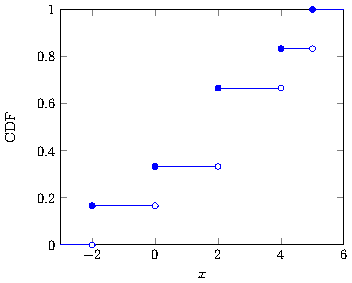
\includegraphics{tikz/figure1}
\end{minipage}%
\begin{minipage}{.5\textwidth}
  \centering
  
\includegraphics{tikz/figure2}
\end{minipage}
\caption{%
(Left) Cumulative Distribution Function (CDF) of a discrete r.v.; 
(Right) CDF of a continuous r.v.}
\end{figure}

For discrete r.v.s, 
the CDF is awkward to work with because of its jumpiness, 
and its derivative is almost useless since it's undefined at 
the jumps and 0 everywhere else. 
But for continuous r.v.s, 
the CDF is often more convenient to work with, 
and its derivative is a very useful function, 
called the \emph{probability density function}.

\emph{Probability density function}. 
For a continuous r.v. \(X\) with CDF \(F\), 
the probability density function (PDF) of \(X\) is the derivative \(f\) of the CDF, 
given by \(f(x) = F^{\prime}(x)\). 
The support of \(X\), and of its distribution, 
is the set of all \(x\) where
\(f(x) > 0\).

An important way in which continuous r.v.s differ from discrete r.v.s 
is that for a continuous r.v. \(X\), 
\(P(X = x) = 0\) for all \(x\). 
This is because \(P(X = x)\) is the height of a jump in the CDF at \(x\), 
but the CDF of \(X\) has no jumps! 
Since the PMF of a continuous r.v. would just be 0 everywhere, 
we work with a PDF instead. 
(This can also be seen by calculating the naïve probability of a sample space \(S=\mathbb{R}\).)

The PDF is analogous to the PMF in many ways, 
but there is a key difference: for a PDF \(f\), 
the quantity \(f(x)\) is \emph{not a probability}, 
and in fact it is possible to have \(f(x) > 1\) for some values of \(x\). 
To obtain a probability, 
we need to \emph{integrate} the PDF. 
The fundamental theorem of calculus tells us how to get from the PDF back to the CDF.

\emph{PDF to CDF}. 
Let \(X\) be a continuous r.v. with PDF \(f\). 
Then the CDF of \(X\) is given by
\begin{align}
F(x) = \int_{- \infty}^{x}{f(t)}dt
\end{align}
The proof is omitted.

\subsection{Intuition}

\subsubsection{Units}

Let \(F\) be the CDF and \(f\) be the PDF of a continuous r.v. \(X\). 
As mentioned earlier, 
\(f(x)\) is not a probability; 
for example, we could have \(f(3) > 1\), and we know \(P(X = 3) = 0\). 
But thinking about the probability of \(X\) being very close to 3 gives us a way to interpret \(f(3)\). 
Specifically, the probability of \(X\) being in a tiny interval of length \(\varepsilon\),
centred at 3, will essentially be \(f(3) \cdot \varepsilon\). 
This is because,
\begin{align}
P(3 - \varepsilon/2 < X < 3 + \varepsilon/2) = 
\int_{3 - \varepsilon/2}^{3 + \varepsilon/2}{f(x)}dx \approx f(3) \cdot \varepsilon
\end{align}
if the interval is so tiny that \(f\) is approximately the constant \(f(3)\) on that interval. 
In general, 
we can think of \(f(x)dx\) as the probability of \(X\) being in 
an infinitesimally small interval containing \(x\), of length \(dx\).

In practice, 
\(X\) often has units in some system of measurement, 
such as units of distance, time, area, or mass. 
Thinking about the units is not only important in applied problems, 
but also it often helps in checking that answers make sense.

Suppose for concreteness that \(X\) is a length, 
measured in centimetres (cm). 
Then \(f(x) = dF(x)/dx\) is the probability per cm at \(x\), 
which explains why \(f(x)\) is a probability density. 
Probability is a dimensionless quantity (a number without physical units), 
so the units of \(f(x)\) are per-cm. 
Therefore, to get a probability again, 
we need to multiply \(f(x)\) by a length. 
When we do an integral such as \(f(x) \cdot dx\), 
this is achieved by the \(dx\).

\begin{figure}[h!]
\centering
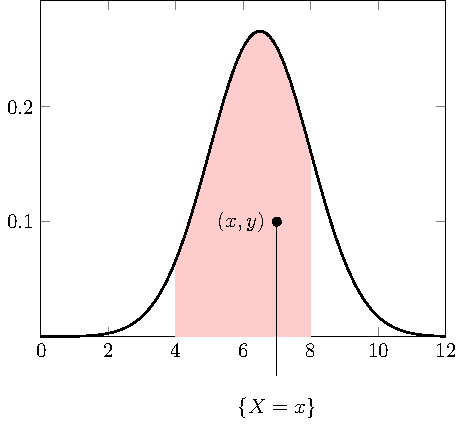
\includegraphics[width=0.5\linewidth]{tikz/figure3}
\caption{%
Uniformly sampling a random point \((x,y)\) under the curve 
and letting \(X=x\) generates an r.v., \(X\), with this PDF.
}
\label{fig:generator}
\end{figure}

\subsubsection{Simulation} 

Another way to think about PDFs is to consider them as generators of the process \(X\). 
To generate \(X\), 
choose a uniformly random point under the PDF curve;
this means that the probability of any region under the curve is the area of that region. 
Then let \(X\) be the \(x\)-coordinate of the random point. 
\(X\) then has the desired distribution since, 
by construction, 
\(P(a \leq X \leq b)\) is the area under the PDF curve 
between the lines \(x = a\) and \(x = b\). 
Thinking about this method helps build intuition for PDFs, 
how random variables are sampled according to a particular PDF curve.

\emph{Question}. 
Use the simulation intuition to describe the 
probability of falling in an interval \([a, b]\) given a
constant PDF (that of continuous uniform random variable).

\subsection{Probability Spaces}

In the previous section we showed that 
intuitively there are several ways to think about 
continuous random variables and their distributions.
The paradoxes that arise when calculating probabilities in a naïve sense
were addressed by the Soviet mathematician Andrey Kolmogorov in the
1930s by introducing the notion of a \emph{probability space}, 
together with other axioms of probability 
(see the session notes on the axioms of probability). 
For most (but not all) practical applications, 
the standard probability space is assumed (and omitted from calculations).

\subsection{Discussion}
\emph{What's the point of learning this? When will we ever come across
these examples in practice -- they aren't applicable in the ``real world''}.

This text provides \emph{definitions} of the concepts with examples that
illustrate -- \emph{in the simplest possible terms} -- what each concept looks like in practice. 
As an analogy, 
when learning how to add and subtract we don't start by 
balancing the accounting books of a multinational corporation. 
We start with simple examples that build an intuitive foundation and build on those 
foundations until we are ready to perform sophisticated accounting tasks. 
(Note, reducing accounting to addition and subtraction is equivalent to reducing 
statistics to calculating conditional probabilities 
-- it's the contextual understanding around the calculations that makes it hard!)

\section{Appendix}

\subsection{Longhand Notation}

In writing \(P(X = x)\), 
we are using \(X = x\) to denote an \emph{event}, 
consisting of all outcomes \(s\) to which \(X\) assigns the number \(x\). 
This event is also written as \(\{ X = x\}\);
formally, \(\{ X = x\}\) is \emph{defined} as \(\{s \in S: X(s) = x\}\), 
read as `` ...the set where each element (outcome) \(s\) in the set (of all possible outcomes) \(S\), 
satisfies the property (mapping) \(X(s) = x\).'' 
But writing \(\{ X = x\}\) is shorter and more intuitive. 

If \(X\) is the number of heads in two fair coin tosses, 
then \(\{ X = 1\}\) consists of the sample outcomes \(HT\) and \(TH\), 
which are the two outcomes to which \(X\) assigns the number 1. 
Since \(\{HT, TH\}\) is a subset of the sample space, 
it is an event. 
So, it makes sense to talk about \(P(X = 1)\), 
or more generally, \(P(X = x)\). 
If \(\{ X = x\}\) were anything other than an event, 
it would make no sense to calculate its probability! 
It does not make sense to write ``\(P(X)\)''; 
we can only take the probability of an event, 
not of a random variable.

\subsection{The Law of the Unconscious Statistician}

\emph{The Law of the Unconscious Statistician}. 
If \(X\) is a discrete r.v. and \(g\) is a function from \(\mathbb{R}\) to \(\mathbb{R}\), then,
\begin{align}
E(g(X)) = \sum_{x}{g(X)}P(X = x)
\end{align}
where \(E(\cdot)\) is the \emph{mathematical expectation} and­ the sum is
taken over all possible values of \(X\).
This means that we can get the expected value of \(g(X)\) knowing only \(P(X = x)\), 
the PMF of \(X\); 
we don't need to know the PMF of \(g(X)\). 
The name comes from the fact that in going from \(E(X)\) to
\(E(g(X))\) it is tempting just to change \(x\) to \(g(x)\) in the definition, 
which can be done very easily and mechanically, 
perhaps in a state of unconsciousness.

On second thought, 
it may sound too good to be true that finding the 
distribution of \(g(X)\) is not needed for this calculation, 
but LOTUS says it is true! 
Before proving LOTUS in general, 
let's see why it is true in some special cases.

Let \(X\) have support 0, 1, 2, \ldots with probabilities \(p_{0}\),
\(p_{1}\), \(p_{2}\), \ldots, so the PMF is \(P(X = n) = p_{n}\). 
Then \(X^{3}\) has support 0, 1, \(2^{3}\), \(2^{4}\), \ldots{} with
probabilities \(p_{0}\), \(p_{1}\), \(p_{2}\), \ldots, so
\begin{align}
E(X) = \sum_{n = 0}^{\infty}{np_{n}},
\end{align}
and
\begin{align}
E\left(X^{3}\right) = \sum_{n = 0}^{\infty}{n^{3}p_{n}}.
\end{align}
As claimed by LOTUS, 
to edit the expression for \(E(X)\) into an expression for \(E(X^{3}\)), 
we can just change the \(n\) in front of the \(p_{n}\) to an \(n^{3}\). 
This was an easy example since the function \(g(x) = x\) is one-to-one. 
But LOTUS holds much more generally. 
The key insight needed for the proof of LOTUS for general
\(g\) is the same as the proof of linearity: the expectation of \(g(X)\)
can be written in ungrouped form as
\begin{align}
E(g(X)) = \sum_{s}{g(X(s))P(\{ s\})},
\end{align}
where the sum is over all the elements in the sample space, 
but we can also group the elements into groups of elements according to the value
that \(X\) assigns to them. 
Within group \(X = x\), 
\(g(X)\) always takes on the value \(g(x)\). 
Therefore, \(E(g(X)) = X\).
In the last step, we used the fact that
\(\sum_{s:X(s) = x}{P\left(\{s\} \right)}\) is the
weight of the group \(X = x\).

\end{document}
